%%%%%%%%%%%%%%%%%%%%%%%%%%%%%%%%%%%%%%%%%%%%%%%%%%%%%%%%%%%%%%%%%%%%%%%%%%%%%%%%%%%%%%%%%%%%%
\chapter{Excess intersection formula}\label{chap:excess_intersection_formula}
Finally, we are able to compute the convolution structure of the Steinberg variety in Theorem \ref{thm:Demazure_operator_1}. We first introduce the convolution product, then give an explicit intersection formula, and finally apply theorems to our settings.

\section{Convolution}\label{sec:convolution}
The construction of the convolution product is similar to a Fourier-Mukai transformation, which is the composition of pullback, tensor product and proper pushforward.

\begin{defn}[Convolution product]\label{def:convolution_product}
For the convenience of reading, we divide the whole process into three steps.
\paragraph*{\underline{Step1.}}Setting.\\[-3mm]

Let $M_1$, $M_2$, $M_3$ be smooth quasi-projective $G$-varieties. For convenience, let
$$M_{ij}:=M_i \times M_j \qquad M_{123}=M_1 \times M_2 \times M_3$$
and $p_i^{jk}, p_i:=p_i^{123}, p_{ij}:=p_{ij}^{123}$ be projections onto some factors, as follows.
% https://q.uiver.app/?q=WzAsNyxbMiwwLCJHIFxcdGltZXMgRyBcXHRpbWVzIFgiXSxbMSwxLCJHIFxcdGltZXMgRyJdLFszLDEsIkcgXFx0aW1lcyBYIl0sWzUsMSwiRyBcXHRpbWVzIFgiXSxbNCwyLCJYIl0sWzIsMiwiRyJdLFswLDIsIkciXSxbMSw2LCJwXzFeezEyfSIsMl0sWzAsMSwicF97MTJ9IiwyXSxbMCwyLCJwX3syM30iXSxbMiw0LCJwXzNeezIzfSJdLFsxLDUsInBfMl57MTJ9Il0sWzIsNSwicF8yXnsyM30iLDJdLFszLDQsInBfM157MTN9IiwwLHsibGFiZWxfcG9zaXRpb24iOjMwLCJzdHlsZSI6eyJib2R5Ijp7Im5hbWUiOiJkYXNoZWQifX19XSxbMyw2LCJwXzFeezEzfSIsMix7ImxhYmVsX3Bvc2l0aW9uIjoyMCwic3R5bGUiOnsiYm9keSI6eyJuYW1lIjoiZGFzaGVkIn19fV0sWzAsMywicF97MTN9IiwwLHsiY3VydmUiOi0yfV1d
\[\begin{tikzcd}[column sep={1.5cm,between origins}]
	&& {M_{123}} &&&[2cm]\\
	& {M_{12}} && {M_{23}} && {M_{13}} \\
	M_1 && M_2 && M_3 &
	\arrow["{p_1^{12}}"', from=2-2, to=3-1]
	\arrow["{p_{12}}"', from=1-3, to=2-2]
	\arrow["{p_{23}}", from=1-3, to=2-4]
	\arrow["{p_3^{23}}", from=2-4, to=3-5]
	\arrow["{p_2^{12}}", from=2-2, to=3-3]
	\arrow["{p_2^{23}}"', from=2-4, to=3-3]
	\arrow["{p_3^{13}}"{pos=0.3}, dashed, from=2-6, to=3-5]
	\arrow["{p_1^{13}}"'{pos=0.2}, dashed, from=2-6, to=3-1]
	\arrow["{p_{13}}", curve={height=-12pt}, from=1-3, to=2-6]
\end{tikzcd}\]
%(Check that $p_i = p_i^{jk} \circ p_{jk}$ for $1 \leqslant j < k \leqslant 3$, $i=j$ or $i=k$)



\paragraph*{\underline{Step2.}}Convolution product on the level of varieties.\\[-3mm]

For closed $G$-subvarieties $Z_{12} \subseteq M_{12}$, $Z_{23} \subseteq M_{23}$, let
$$Z_{123}:= p_{12}^{-1}(Z_{12}) \cap p_{23}^{-1}(Z_{23}) \subseteq M_{123}$$
be the intersection of two preimages. The \textbf{convolution product} of $Z_{12}$ and $Z_{23}$ is defined as
$$Z_{12} \circ Z_{23} := p_{13}(Z_{123}) \subseteq M_{13}$$
which is a closed $G$-subvariety of $M_{13}$.
\paragraph*{\underline{Step3.}}Convolution product on the level of $K$-theories.\\[-3mm]

Let 
$$\pi_{12}:=p_{12}\big|_{p_{12}^{-1}(Z_{12})} \qquad \pi_{23}:=p_{23}\big|_{p_{23}^{-1}(Z_{23})} \qquad
\pi_{13}:=p_{13}\big|_{Z_{123}}$$
be corresponding morphisms restricted to $p_{12}^{-1}(Z_{12})$, $p_{23}^{-1}(Z_{23})$ and  $Z_{123}$, respectively. We assume that $\pi_{13}$ is proper, so that we can use proper pushforward in $K$-theory.

We define the convolution product by
$$*: K_0^G(Z_{12}) \times K_0^G(Z_{23}) \longrightarrow K_0^G(Z_{12} \circ Z_{23}) \qquad (\mathcal{F}_{12}, \mathcal{F}_{23}) \longmapsto \mathcal{F}_{12}*\mathcal{F}_{23}$$
$$\mathcal{F}_{12}*\mathcal{F}_{23}=\pi_{13,*}\left(\pi_{12}^* \mathcal{F}_{12} \otimes \pi_{23}^* \mathcal{F}_{23} \right) \in K_0^G(Z_{12} \circ Z_{23})$$

\end{defn}

\begin{remark}
Those ``$Z$-varieties" ($Z_{12}$, $p_{12}^{-1}(Z_{12})$, $Z_{123}$, etc.) are often singular in practice, so $\pi_{12}^{*}$, $\pi_{23}^{*}$ and $\otimes$ are defined in the sense of ``restriction with supports", under the ``$M$-varieties" which are smooth. The following diagram best illustrates the ``actual" definition.
%closed immersion induce f.faithful map in quasicoherent sheaf: https://en.wikipedia.org/wiki/Closed_immersion
% https://q.uiver.app/?q=WzAsOCxbMCwwLCJLXzBeRyhaX3sxMn0pIFxcdGltZXMgS18wXkcoWl97MjN9KSJdLFsxLDAsIktfMF5HXFxiaWcocF97MTJ9XnstMX0oWl97MTJ9KVxcYmlnKSBcXHRpbWVzIEtfMF5HXFxiaWcocF97MTJ9XnstMX0oWl97MjN9KVxcYmlnKSJdLFswLDEsIktfMF5HKE1fezEyfSkgXFx0aW1lcyBLXzBeRyhNX3syM30pIl0sWzEsMSwiS18wXkcoTV97MTIzfSkgXFx0aW1lcyBLXzBeRyhNX3sxMjN9KSJdLFsyLDEsIktfMF5HKE1fezEyM30pIl0sWzMsMSwiS18wXkcoTV97MTN9KSJdLFsyLDAsIktfMF5HKFpfezEyM30pIl0sWzMsMCwiS18wXkcoWl97MTJ9IFxcY2lyYyBaX3syM30pIl0sWzAsMiwiIiwwLHsic3R5bGUiOnsidGFpbCI6eyJuYW1lIjoiaG9vayIsInNpZGUiOiJib3R0b20ifX19XSxbMSwzLCIiLDAseyJzdHlsZSI6eyJ0YWlsIjp7Im5hbWUiOiJob29rIiwic2lkZSI6ImJvdHRvbSJ9fX1dLFs2LDQsIiIsMCx7InN0eWxlIjp7InRhaWwiOnsibmFtZSI6Imhvb2siLCJzaWRlIjoiYm90dG9tIn19fV0sWzcsNSwiIiwwLHsic3R5bGUiOnsidGFpbCI6eyJuYW1lIjoiaG9vayIsInNpZGUiOiJib3R0b20ifX19XSxbMiwzLCJwX3sxMn1eKiBcXHRpbWVzIHBfezIzfV4qIl0sWzMsNCwiXFxvdGltZXMiXSxbNCw1LCJwX3sxMywqfSJdLFs2LDcsIlxccGlfezEzLCp9Il0sWzEsNiwiXFxvdGltZXMiLDAseyJzdHlsZSI6eyJib2R5Ijp7Im5hbWUiOiJkYXNoZWQifX19XSxbMCwxLCJcXHBpX3sxMn1eKiBcXHRpbWVzIFxccGlfezIzfV4qIiwwLHsic3R5bGUiOnsiYm9keSI6eyJuYW1lIjoiZGFzaGVkIn19fV1d
\tikzcdset{scale cd/.style={every label/.append style={scale=#1},
    cells={nodes={scale=#1}}}}
\begin{equation}\label{eq:convolution_singularity_solved}
\begin{tikzcd}[scale cd=0.7]
	{K_0^G(Z_{12}) \times K_0^G(Z_{23})} & {K_0^G\big(p_{12}^{-1}(Z_{12})\big) \times K_0^G\big(p_{12}^{-1}(Z_{23})\big)} & {K_0^G(Z_{123})} & {K_0^G(Z_{12} \circ Z_{23})} \\
	{K_0^G(M_{12}) \times K_0^G(M_{23})} & {K_0^G(M_{123}) \times K_0^G(M_{123})} & {K_0^G(M_{123})} & {K_0^G(M_{13})}
	\arrow["{\iota_{Z_{12},*}, \iota_{Z_{23},*}}",from=1-1, to=2-1]
	\arrow[from=1-2, to=2-2]
	\arrow[from=1-3, to=2-3]
	\arrow["{\iota_{Z_{12} \circ Z_{23},*}}"', from=1-4, to=2-4]
	\arrow["{p_{12}^* \times p_{23}^*}", from=2-1, to=2-2]
	\arrow["\otimes", from=2-2, to=2-3]
	\arrow["{p_{13,*}}", from=2-3, to=2-4]
	\arrow["{\pi_{13,*}}", from=1-3, to=1-4]
	\arrow["\otimes", dashed, from=1-2, to=1-3]
	\arrow["{\pi_{12}^* \times \pi_{23}^*}", dashed, from=1-1, to=1-2]
\end{tikzcd}
\end{equation}
The diagram in \eqref{eq:convolution_singularity_solved} commutes by the vanishing of the Euler class. Therefore, one can compute
$$\mathcal{F}_{12}*\mathcal{F}_{23}=p_{13,*}\left(p_{12}^* \iota_{Z_{12},*}\mathcal{F}_{12} \otimes p_{23}^* \iota_{Z_{23},*}\mathcal{F}_{23} \right) \in K_0^G(M_{13}),$$
and then find the preimage of it under the map $\iota_{Z_{12} \circ Z_{23},*}$. This technique will be used in Subsection \ref{subsec:convolution_product_fml}.
\end{remark}

The whole process can be concluded in Figure \ref{fig:convolution_product}.
\begin{figure}[ht]
  \vspace{0cm}
    \centering  
    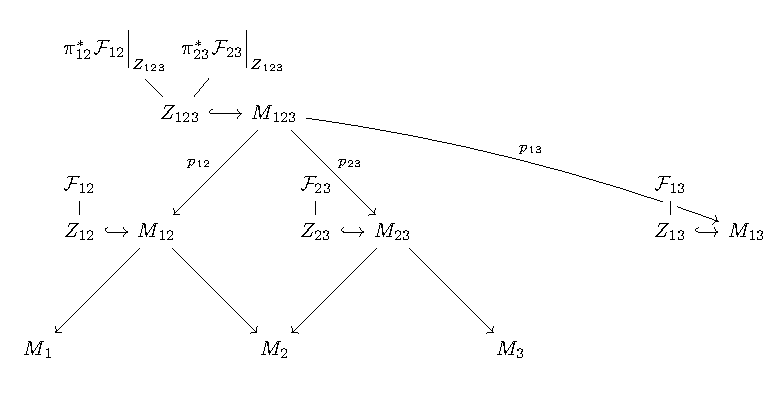
\includegraphics[]{figures/table/figure_convolution.pdf}    
    \caption{Convolution Product}  
    \label{fig:convolution_product}
\end{figure}

\section{Statement}
To facilitate the computation of intersections (i.e., tensor product in the construction of convolution product), we state the excess intersection formula.

\begin{theorem}[{Excess intersection formula, \cite[Corollary 9.4]{przezdziecki2015geometric}}]\label{thm:excess_intersection_formula}
Let $X'$ be a smooth $G$-variety, $X \subseteq X'$ be a (maybe singular) closed $G$-subvariety, and $Y_1,Y_2 \subseteq X$ be closed $G$-equivariant embeddings (of globally finite $\Tor$-dimension). Denote
\begin{equation*}
\begin{aligned}
  Y:=\;&Y_1 \cap Y_2 \qquad \iota_Y: Y \hookrightarrow X  \\
  \mathcal{T}:=\;&TX\big|_{Y} / \left( TY_1\big|_{Y}+ TY_2\big|_{Y}   \right) 
\end{aligned}
\end{equation*}
\begin{equation}\label{eq:excess_intersection_formula}
% https://q.uiver.app/?q=WzAsNyxbMSwxLCJXIl0sWzMsMSwiWiJdLFszLDIsIlgiXSxbMSwyLCJZIl0sWzQsMCwiXFxtYXRoY2Fse059X3tcXHZhcnBoaX0iXSxbMiwwLCJnXnsqfVxcbWF0aGNhbHtOfV97XFx2YXJwaGl9Il0sWzAsMCwiXFxtYXRoY2Fse059X3tcXHBoaX0iXSxbMywyLCJmIl0sWzEsMiwiXFx2YXJwaGkiXSxbMCwxLCJnIl0sWzAsMywiXFxwaGkiLDJdLFs0LDEsIiIsMCx7InN0eWxlIjp7ImhlYWQiOnsibmFtZSI6Im5vbmUifX19XSxbNSwwLCIiLDAseyJzdHlsZSI6eyJoZWFkIjp7Im5hbWUiOiJub25lIn19fV0sWzYsMCwiIiwwLHsic3R5bGUiOnsiaGVhZCI6eyJuYW1lIjoibm9uZSJ9fX1dXQ==
\begin{tikzcd}[row sep={between origins,20mm},column sep={between origins,5mm}]
	{N_Y Y_2} &[3mm]&[3mm] {\frac{N_Y X}{N_Y Y_1}} &[10mm]&[3mm] {N_{Y_1}X} \\[-9mm]
	& Y && Y_1 \\
	& Y_2 && X
	\arrow["f", from=3-2, to=3-4]
	\arrow["\varphi", from=2-4, to=3-4]
	\arrow["g", from=2-2, to=2-4]
	\arrow["\phi"', from=2-2, to=3-2]
	\arrow[no head, from=1-5, to=2-4]
	\arrow[no head, from=1-3, to=2-2]
	\arrow[no head, from=1-1, to=2-2]
\end{tikzcd}
\end{equation}
Assume that $TY_1\big|_{Y} \cap TY_2\big|_{Y} = TY$. We get the  excess intersection formula:
$$[Y_1]_{X}^G \otimes [Y_2]_{X}^G = \iota_{Y,*} \left(\eu( \mathcal{T} ) \cdot [Y]_{Y}^G \right).$$
In particular, when $Y=\pt$ is a point, we get simplified formula in $K^G(X)$:
$$[Y_1]^G \otimes [Y_2]^G = \eu( \mathcal{T} ) \cdot [Y]^G $$
where $\eu( \mathcal{T} ) \in \Rpt(G)$ acts by scalar multiplication.
\end{theorem}

Readers may find Theorem \ref{thm:excess_intersection_formula} as a special case of excess base change theorem. In fact,
\begin{equation*}
\begin{aligned}\
   [Y_1]_{X}^G \otimes [Y_2]_{X}^G=\;& [Y_1]_{X}^G \otimes f_*[Y_2]_{Y_2}^G&& \text{definition of $[Y_2]_{X}^G$}\\
   =\;& f_*\left(f^*[Y_1]_{X}^G \otimes [Y_2]_{Y_2}^G\right) && \text{proper projection formula}\\
   =\;& f_*\left(f^*[Y_1]_{X}^G \right) && \text{Lemma \ref{lem:unit_of_tensor_product}}\\
   =\;& f_*\left(f^*\varphi_{*}[Y_1]_{Y_1}^G \right) && \text{definition of $[Y_1]_{X}^G$}\\
   =\;& f_*\left(\phi_{*} \left( \eu(\mathcal{T})\cdot g^*[Y_1]_{Y_1}^G\rule{0mm}{3.6mm}  \right)\rule{0mm}{4mm} \right) && \text{excess base change to \eqref{eq:excess_intersection_formula}}\\
   =\;& \iota_{Y,*} \left(\eu( \mathcal{T} ) \cdot [Y]_{Y}^G \right) &&\\
\end{aligned}
\end{equation*}

The projection formula is stated here.
\begin{proposition}[Projection formula]
For any proper $G$-equivariant morphism $f:Y \longrightarrow X$ of globally finite $\Tor$-dimension, $\alpha \in K^G(Y)$, $\beta \in K^G(X)$, we have proper projection formula:
$$f_* \alpha \otimes \beta =f_*(\alpha \otimes f^{*} \beta).$$
\end{proposition}

\section{Application: convolution structure}
In this section, we will apply Definition \ref{def:convolution_product} and Theorem \ref{thm:excess_intersection_formula} to our typical varieties. In particular, we will get the convolution product formula in terms of basis elements $\preimage{\phi}_{\ww}$ and $\preimage{\phi}_{\ww,\ww'}$.

\subsection{Algebraic structures induced by convolution product}

\begin{defn}[Convolution product structure on $K^{G_{\dimvec{d}}}(\St_{\dimvec{d}})$]
Following notations in \ref{def:convolution_product}, We take $G=G_{\dimvec{d}}$,
\begin{equation*}
\begin{aligned}
  M_1=\;& M_2=M_3= \RRep_{\dimvec{d}}(Q) \\ 
  Z_{12}=\;& Z_{23}= \St_{\dimvec{d}} \\ 
  \St_{\dimvec{d}}=\;& \RRep_{\dimvec{d}}(Q) \times_{\Rep_{\dimvec{d}}(Q)} \RRep_{\dimvec{d}}(Q) \subseteq \RRep_{\dimvec{d}}(Q) \times \RRep_{\dimvec{d}}(Q)
\end{aligned}
\end{equation*}
By definition, we see that $\St_{\dimvec{d}} \circ \St_{\dimvec{d}} = \St_{\dimvec{d}}$. Therefore, we define a ring structure on $K^{G_{\dimvec{d}}}(\St_{\dimvec{d}})$:
$$\fakestar: K^{G_{\dimvec{d}}}(\St_{\dimvec{d}}) \times K^{G_{\dimvec{d}}}(\St_{\dimvec{d}}) \longrightarrow K^{G_{\dimvec{d}}}(\St_{\dimvec{d}}).$$
\end{defn}

\begin{defn}[$K^{G_{\dimvec{d}}}(\St_{\dimvec{d}})$-module structure on $K^{G_{\dimvec{d}}}(\RRep_{\dimvec{d}}(Q))$]
Following notations in \ref{def:convolution_product}, We take $G=G_{\dimvec{d}}$,
\begin{equation*}
\begin{aligned}
  M_1=\;& M_2= \RRep_{\dimvec{d}}(Q)  \qquad& M_3=\;& \{\pt\}\\ 
  Z_{12}=\;& \St_{\dimvec{d}} & Z_{23}=\;& \RRep_{\dimvec{d}}(Q) \\ 
\end{aligned}
\end{equation*}
By definition, we see that $\St_{\dimvec{d}} \circ \RRep_{\dimvec{d}}(Q) = \RRep_{\dimvec{d}}(Q)$. Therefore, we define a $K^{G_{\dimvec{d}}}(\St_{\dimvec{d}})$-module structure on $K^{G_{\dimvec{d}}}\left(\RRep_{\dimvec{d}}(Q)\right)$:
$$\star: K^{G_{\dimvec{d}}}(\St_{\dimvec{d}}) \times K^{G_{\dimvec{d}}}\left(\RRep_{\dimvec{d}}(Q)\right) \longrightarrow K^{G_{\dimvec{d}}}\left(\RRep_{\dimvec{d}}(Q)\right).$$
\end{defn}

\begin{remark}\label{rmk:process_convolution_product}
Notice that in the construction of the convolution product, pullback, tensor product and proper pushforward are compatible with the forgetful map of groups. Therefore, the following diagrams commute:
% https://q.uiver.app/?q=WzAsMTgsWzAsMCwiS157R197XFxkaW12ZWN7ZH19fShcXFN0X3tcXGRpbXZlY3tkfX0pIl0sWzEsMCwiS157R197XFxkaW12ZWN7ZH19fShcXFN0X3tcXGRpbXZlY3tkfX0pIl0sWzIsMCwiS157R197XFxkaW12ZWN7ZH19fShcXFN0X3tcXGRpbXZlY3tkfX0pIl0sWzMsMCwiS157R197XFxkaW12ZWN7ZH19fShcXFN0X3tcXGRpbXZlY3tkfX0pIl0sWzQsMCwiS157R197XFxkaW12ZWN7ZH19fVxcbGVmdChcXFJSZXBfe1xcZGltdmVje2R9fShRKVxccmlnaHQpIl0sWzUsMCwiS157R197XFxkaW12ZWN7ZH19fVxcbGVmdChcXFJSZXBfe1xcZGltdmVje2R9fShRKVxccmlnaHQpIl0sWzAsMSwiS157VF97XFxkaW12ZWN7ZH19fShcXFN0X3tcXGRpbXZlY3tkfX0pIl0sWzEsMSwiS157VF97XFxkaW12ZWN7ZH19fShcXFN0X3tcXGRpbXZlY3tkfX0pIl0sWzIsMSwiS157VF97XFxkaW12ZWN7ZH19fShcXFN0X3tcXGRpbXZlY3tkfX0pIl0sWzMsMSwiS157VF97XFxkaW12ZWN7ZH19fShcXFN0X3tcXGRpbXZlY3tkfX0pIl0sWzQsMSwiS157VF97XFxkaW12ZWN7ZH19fVxcbGVmdChcXFJSZXBfe1xcZGltdmVje2R9fShRKVxccmlnaHQpIl0sWzUsMSwiS157VF97XFxkaW12ZWN7ZH19fVxcbGVmdChcXFJSZXBfe1xcZGltdmVje2R9fShRKVxccmlnaHQpIl0sWzAsMiwiXFxLY3VybF57VF97XFxkaW12ZWN7ZH19fShcXFN0X3tcXGRpbXZlY3tkfX0pIl0sWzEsMiwiXFxLY3VybF57VF97XFxkaW12ZWN7ZH19fShcXFN0X3tcXGRpbXZlY3tkfX0pIl0sWzIsMiwiXFxLY3VybF57VF97XFxkaW12ZWN7ZH19fShcXFN0X3tcXGRpbXZlY3tkfX0pIl0sWzMsMiwiXFxLY3VybF57VF97XFxkaW12ZWN7ZH19fShcXFN0X3tcXGRpbXZlY3tkfX0pIl0sWzQsMiwiXFxLY3VybF57VF97XFxkaW12ZWN7ZH19fVxcbGVmdChcXFJSZXBfe1xcZGltdmVje2R9fShRKVxccmlnaHQpIl0sWzUsMiwiXFxLY3VybF57VF97XFxkaW12ZWN7ZH19fVxcbGVmdChcXFJSZXBfe1xcZGltdmVje2R9fShRKVxccmlnaHQpIl0sWzAsNiwiIiwwLHsic3R5bGUiOnsidGFpbCI6eyJuYW1lIjoiaG9vayIsInNpZGUiOiJib3R0b20ifX19XSxbMSw3LCIiLDAseyJzdHlsZSI6eyJ0YWlsIjp7Im5hbWUiOiJob29rIiwic2lkZSI6ImJvdHRvbSJ9fX1dLFsyLDgsIiIsMCx7InN0eWxlIjp7InRhaWwiOnsibmFtZSI6Imhvb2siLCJzaWRlIjoiYm90dG9tIn19fV0sWzMsOSwiIiwwLHsic3R5bGUiOnsidGFpbCI6eyJuYW1lIjoiaG9vayIsInNpZGUiOiJib3R0b20ifX19XSxbNCwxMCwiIiwwLHsic3R5bGUiOnsidGFpbCI6eyJuYW1lIjoiaG9vayIsInNpZGUiOiJib3R0b20ifX19XSxbNiwxMiwiIiwwLHsic3R5bGUiOnsidGFpbCI6eyJuYW1lIjoiaG9vayIsInNpZGUiOiJib3R0b20ifX19XSxbNywxMywiIiwwLHsic3R5bGUiOnsidGFpbCI6eyJuYW1lIjoiaG9vayIsInNpZGUiOiJib3R0b20ifX19XSxbOCwxNCwiIiwwLHsic3R5bGUiOnsidGFpbCI6eyJuYW1lIjoiaG9vayIsInNpZGUiOiJib3R0b20ifX19XSxbOSwxNSwiIiwwLHsic3R5bGUiOnsidGFpbCI6eyJuYW1lIjoiaG9vayIsInNpZGUiOiJib3R0b20ifX19XSxbMTAsMTYsIiIsMCx7InN0eWxlIjp7InRhaWwiOnsibmFtZSI6Imhvb2siLCJzaWRlIjoiYm90dG9tIn19fV0sWzUsMTEsIiIsMCx7InN0eWxlIjp7InRhaWwiOnsibmFtZSI6Imhvb2siLCJzaWRlIjoiYm90dG9tIn19fV0sWzExLDE3LCIiLDAseyJzdHlsZSI6eyJ0YWlsIjp7Im5hbWUiOiJob29rIiwic2lkZSI6ImJvdHRvbSJ9fX1dLFs0LDUsIlxcZGl2aWRlb250aW1lcyJdLFsxMCwxMSwiXFxkaXZpZGVvbnRpbWVzIl0sWzE2LDE3LCJcXGRpdmlkZW9udGltZXMiXSxbMSwyLCIqIl0sWzcsOCwiKiJdLFsxMywxNCwiKiJdLFszLDQsIlxcdGltZXMiLDEseyJzdHlsZSI6eyJib2R5Ijp7Im5hbWUiOiJub25lIn0sImhlYWQiOnsibmFtZSI6Im5vbmUifX19XSxbOSwxMCwiXFx0aW1lcyIsMSx7InN0eWxlIjp7ImJvZHkiOnsibmFtZSI6Im5vbmUifSwiaGVhZCI6eyJuYW1lIjoibm9uZSJ9fX1dLFsxNSwxNiwiXFx0aW1lcyIsMSx7InN0eWxlIjp7ImJvZHkiOnsibmFtZSI6Im5vbmUifSwiaGVhZCI6eyJuYW1lIjoibm9uZSJ9fX1dLFswLDEsIlxcdGltZXMiLDEseyJzdHlsZSI6eyJib2R5Ijp7Im5hbWUiOiJub25lIn0sImhlYWQiOnsibmFtZSI6Im5vbmUifX19XSxbNiw3LCJcXHRpbWVzIiwxLHsic3R5bGUiOnsiYm9keSI6eyJuYW1lIjoibm9uZSJ9LCJoZWFkIjp7Im5hbWUiOiJub25lIn19fV0sWzEyLDEzLCJcXHRpbWVzIiwxLHsic3R5bGUiOnsiYm9keSI6eyJuYW1lIjoibm9uZSJ9LCJoZWFkIjp7Im5hbWUiOiJub25lIn19fV1d
\[\begin{tikzcd}
	{K^{G_{\dimvec{d}}}(\St_{\dimvec{d}})} &[-9mm] {K^{G_{\dimvec{d}}}(\St_{\dimvec{d}})} &[-3mm] {K^{G_{\dimvec{d}}}(\St_{\dimvec{d}})} &[-3mm] {K^{G_{\dimvec{d}}}(\St_{\dimvec{d}})} &[-9mm] {K^{G_{\dimvec{d}}}\left(\RRep_{\dimvec{d}}(Q)\right)} &[-3mm] {K^{G_{\dimvec{d}}}\left(\RRep_{\dimvec{d}}(Q)\right)} \\
	{K^{T_{\dimvec{d}}}(\St_{\dimvec{d}})} & {K^{T_{\dimvec{d}}}(\St_{\dimvec{d}})} & {K^{T_{\dimvec{d}}}(\St_{\dimvec{d}})} & {K^{T_{\dimvec{d}}}(\St_{\dimvec{d}})} & {K^{T_{\dimvec{d}}}\left(\RRep_{\dimvec{d}}(Q)\right)} & {K^{T_{\dimvec{d}}}\left(\RRep_{\dimvec{d}}(Q)\right)} \\
	{\Kcurl^{T_{\dimvec{d}}}(\St_{\dimvec{d}})} & {\Kcurl^{T_{\dimvec{d}}}(\St_{\dimvec{d}})} & {\Kcurl^{T_{\dimvec{d}}}(\St_{\dimvec{d}})} & {\Kcurl^{T_{\dimvec{d}}}(\St_{\dimvec{d}})} & {\Kcurl^{T_{\dimvec{d}}}\left(\RRep_{\dimvec{d}}(Q)\right)} & {\Kcurl^{T_{\dimvec{d}}}\left(\RRep_{\dimvec{d}}(Q)\right)}
	\arrow[hook', from=1-1, to=2-1]
	\arrow[hook', from=1-2, to=2-2]
	\arrow[hook', from=1-3, to=2-3]
	\arrow[hook', from=1-4, to=2-4]
	\arrow[hook', from=1-5, to=2-5]
	\arrow[hook', from=2-1, to=3-1]
	\arrow[hook', from=2-2, to=3-2]
	\arrow[hook', from=2-3, to=3-3]
	\arrow[hook', from=2-4, to=3-4]
	\arrow[hook', from=2-5, to=3-5]
	\arrow[hook', from=1-6, to=2-6]
	\arrow[hook', from=2-6, to=3-6]
	\arrow["\star", from=1-5, to=1-6]
	\arrow["\star", from=2-5, to=2-6]
	\arrow["\star", from=3-5, to=3-6]
	\arrow["\fakestar", from=1-2, to=1-3]
	\arrow["\fakestar", from=2-2, to=2-3]
	\arrow["\fakestar", from=3-2, to=3-3]
	\arrow["\times"{description}, draw=none, from=1-4, to=1-5]
	\arrow["\times"{description}, draw=none, from=2-4, to=2-5]
	\arrow["\times"{description}, draw=none, from=3-4, to=3-5]
	\arrow["\times"{description}, draw=none, from=1-1, to=1-2]
	\arrow["\times"{description}, draw=none, from=2-1, to=2-2]
	\arrow["\times"{description}, draw=none, from=3-1, to=3-2]
\end{tikzcd}\]
\end{remark}

\begin{defn}[$K^{G_{\dimvec{d}}}(\RRep_{\dimvec{d}}(Q))$-module structure on $K^{G_{\dimvec{d}}}(\St_{\dimvec{d}})$]
We know that 
$$\RRep_{\dimvec{d}}(Q) \cong \St_{\Id} \subseteq \St_{\dimvec{d}}, \qquad \St_{\Id} \circ \St_{\Id} = \St_{\Id},$$
so $K^{G_{\dimvec{d}}}\left(\RRep_{\dimvec{d}}(Q)\right)$ can be realized as a $R(G_{\dimvec{d}})$-subalgebra of $K^{G_{\dimvec{d}}}(\St_{\dimvec{d}})$, and $K^{G_{\dimvec{d}}}(\St_{\dimvec{d}})$ has the $K^{G_{\dimvec{d}}}\left(\RRep_{\dimvec{d}}(Q)\right)$-module structure induced by the convolution product:
$$\fakestar: K^{G_{\dimvec{d}}}\left(\RRep_{\dimvec{d}}(Q)\right) \times K^{G_{\dimvec{d}}}(\St_{\dimvec{d}}) \longrightarrow K^{G_{\dimvec{d}}}(\St_{\dimvec{d}}).$$
\end{defn}

\subsection{Convolution product formula}\label{subsec:convolution_product_fml}


In this subsection, we compute the convolution product in the bottom line of the diagram in Remark \ref{rmk:process_convolution_product}.
\begin{proposition}[Convolution product formula]\label{prop:convolution_product_formula}
For $\ww$, $\ww'$, $\ww''$, $\ww''' \in \WWd$, we have
\begin{equation*}
\begin{aligned}
  \preimage{\psi}_{\ww,\ww'} \fakestar \preimage{\psi}_{\ww'',\ww'''}=\;& \delta_{\ww',\ww''}\preimage{\Lambda}_{\ww'} \preimage{\psi}_{\ww,\ww'''} \\ 
  \preimage{\psi}_{\ww,\ww'} \star \preimage{\psi}_{\ww''\phantom{,\ww'''}}=\;& \delta_{\ww',\ww''}\preimage{\Lambda}_{\ww'} \preimage{\psi}_{\ww}. \\   
\end{aligned}
\end{equation*}
\end{proposition}
\begin{proof}
Follow the Definition \ref{def:convolution_product} and Theorem \ref{thm:excess_intersection_formula} if needed.

For clearance, we divide the proof into four cases.

\paragraph*{\underline{Case 1.}}Assume $\ww' \neq \ww''$, need to show $\preimage{\psi}_{\ww,\ww'} \fakestar \preimage{\psi}_{\ww'',\ww'''}=0$.\\[-3mm]

Denote 
%\footnote{For some people, the notation
%$$Y_{12}:= \left\{\rule{0mm}{3mm}\!\left(\rule{0mm}{2.8mm}(\rho_0, F_{\ww}),(\rho_0, F_{\ww'})\right) \right\} \subseteq \St_{\dimvec{d}}$$ is better for understanding. We don't write like that, because too many brackets occupy attentions.
%}
$$Y_{12}:= \{(\rho_0, F_{\ww}, F_{\ww'}) \} \subseteq \St_{\dimvec{d}}, \qquad Y_{23}:= \{(\rho_0, F_{\ww''}, F_{\ww'''}) \} \subseteq \St_{\dimvec{d}}.$$
Since $\ww' \neq \ww''$, $p_{12}^{-1} (Y_{12}) \cap
p_{23}^{-1} (Y_{23}) = \varnothing$, so
\begin{equation*}
\begin{aligned}
\preimage{\psi}_{\ww,\ww'} \fakestar \preimage{\psi}_{\ww'',\ww'''}=\;& \left[ Y_{12}   \right]_{\St_{\dimvec{d}}}^{T_{\dimvec{d}}}  \fakestar \left[ Y_{23}  \right]_{\St_{\dimvec{d}}}^{T_{\dimvec{d}}}\\ 
=\;&p_{13,*}\left(p_{12}^* \left[ Y_{12}   \right]_{M_{12}}^{T_{\dimvec{d}}}  \otimes p_{23}^* \left[ Y_{23}  \right]_{M_{23}}^{T_{\dimvec{d}}} \right)\\
=\;&p_{13,*}\left(\left[ p_{12}^{-1}(Y_{12})   \right]_{M_{123}}^{T_{\dimvec{d}}}  \otimes \left[  p_{12}^{-1}(Y_{23})  \right]_{M_{123}}^{T_{\dimvec{d}}} \right)\\
=\;&0
\end{aligned}
\end{equation*}

\paragraph*{\underline{Case 2.}}Assume $\ww' \neq \ww''$, need to show $\preimage{\psi}_{\ww,\ww'} \star \preimage{\psi}_{\ww''}=0$.\\[-3mm]

Denote
$$Y_{12}:= \{(\rho_0, F_{\ww}, F_{\ww'}) \} \subseteq \St_{\dimvec{d}}, \qquad Y_{23}:= \{(\rho_0, F_{\ww''}) \} \subseteq \RRep_{\dimvec{d}}(Q).$$
Since $\ww' \neq \ww''$, $p_{12}^{-1} (Y_{12}) \cap
p_{23}^{-1} (Y_{23}) = \varnothing$, so
\begin{equation*}
\begin{aligned}
\preimage{\psi}_{\ww,\ww'} \star \preimage{\psi}_{\ww''}=\;& \left[ Y_{12}   \right]_{\St_{\dimvec{d}}}^{T_{\dimvec{d}}}  \star \left[ Y_{23}  \right]_{\RRep_{\dimvec{d}}(Q)}^{T_{\dimvec{d}}}\\ 
=\;&p_{13,*}\left(p_{12}^* \left[ Y_{12}   \right]_{M_{12}}^{T_{\dimvec{d}}}  \otimes p_{23}^* \left[ Y_{23}  \right]_{M_{23}}^{T_{\dimvec{d}}} \right)\\
=\;&p_{13,*}\left(\left[ p_{12}^{-1}(Y_{12})   \right]_{M_{123}}^{T_{\dimvec{d}}}  \otimes \left[  p_{12}^{-1}(Y_{23})  \right]_{M_{123}}^{T_{\dimvec{d}}} \right)\\
=\;&0
\end{aligned}
\end{equation*}

\paragraph*{\underline{Case 3.}}For $\ww$, $\ww'$, $\ww'' \in \WWd$, need to show that $$\preimage{\psi}_{\ww,\ww'} \fakestar \preimage{\psi}_{\ww',\ww''}=\preimage{\Lambda}_{\ww'}\preimage{\psi}_{\ww,\ww''}.$$

Denote 
$$Y_{12}:= \{(\rho_0, F_{\ww}, F_{\ww'}) \} \subseteq \St_{\dimvec{d}}, \qquad Y_{23}:= \{(\rho_0, F_{\ww'}, F_{\ww''}) \} \subseteq \St_{\dimvec{d}},$$
then
\begin{equation*}
\begin{aligned}
  &p_{12}^{-1}(Y_{12})= Y_{12} \times \RRep_{\dimvec{d}}(Q) \qquad & p_{23}^{-1}(Y_{23})=\;&   \RRep_{\dimvec{d}}(Q) \times Y_{23}\\ 
  &p_{12}^{-1}(Y_{12}) \cup p_{23}^{-1}(Y_{23})=Y & Y_{12}\circ Y_{23}=\;&Y_{13},
\end{aligned}
\end{equation*}
where
\begin{equation*}
\begin{aligned}
  &Y=\{y\} \qquad && y=\big( (\rho_0,F_{\ww}),(\rho_0,F_{\ww'}),(\rho_0,F_{\ww''})  \big) & &\in M_{123}  \\ 
  &Y_{13}=\{y_{13}\} \qquad && y_{13}=\big( (\rho_0,F_{\ww}),(\rho_0,F_{\ww''})  \big) & &\in M_{13}.  \\
\end{aligned}
\end{equation*}
Therefore, 
\begin{equation*}
\begin{aligned}
\preimage{\psi}_{\ww,\ww'} \fakestar \preimage{\psi}_{\ww',\ww''}=\;& \left[ Y_{12}   \right]_{\St_{\dimvec{d}}}^{T_{\dimvec{d}}}  \fakestar \left[ Y_{23}  \right]_{\St_{\dimvec{d}}}^{T_{\dimvec{d}}}\\ 
=\;&p_{13,*}\left(p_{12}^* \left[ Y_{12}   \right]_{M_{12}}^{T_{\dimvec{d}}}  \otimes p_{23}^* \left[ Y_{23}  \right]_{M_{23}}^{T_{\dimvec{d}}} \right)\\
=\;&p_{13,*}\left(\left[ p_{12}^{-1}(Y_{12})   \right]_{M_{123}}^{T_{\dimvec{d}}}  \otimes \left[  p_{12}^{-1}(Y_{23})  \right]_{M_{123}}^{T_{\dimvec{d}}} \right)\\
=\;&p_{13,*}\left(\eu( \mathcal{T} ) \cdot [Y]_{M_{123}}^{T_{\dimvec{d}}} \right)\\
=\;&\eu( \mathcal{T} )\cdot [Y]_{M_{13}}^{T_{\dimvec{d}}} \\
=\;& \preimage{\Lambda}_{\ww'}\preimage{\psi}_{\ww,\ww''}
\end{aligned}
\end{equation*}
where
$$\mathcal{T}:= \frac{T_y M_{123} }{T_y \big( p_{12}^{-1}(Y_{12}) \big) \oplus T_y \big( p_{23}^{-1}(Y_{23}) \big)} = \frac{\preimage{\mathcal{T}}_{\ww} \oplus \preimage{\mathcal{T}}_{\ww'} \oplus \preimage{\mathcal{T}}_{\ww''}}{\preimage{\mathcal{T}}_{\ww} \hfill\oplus \hfill  \preimage{\mathcal{T}}_{\ww''}}= \preimage{\mathcal{T}}_{\ww'}.$$
\paragraph*{\underline{Case 4.}}For $\ww$, $\ww' \in \WWd$, need to show that $$\preimage{\psi}_{\ww,\ww'} \star \preimage{\psi}_{\ww'}=\preimage{\Lambda}_{\ww'}\preimage{\psi}_{\ww}.$$

Denote 
$$Y_{12}:= \{(\rho_0, F_{\ww}, F_{\ww'}) \} \subseteq \St_{\dimvec{d}}, \qquad Y_{23}:= \{(\rho_0, F_{\ww'}) \} \subseteq \RRep_{\dimvec{d}}(Q),$$
then
\begin{equation*}
\begin{aligned}
  &p_{12}^{-1}(Y_{12})= Y_{12} \times \{\pt\} \qquad & p_{23}^{-1}(Y_{23})=\;&   \RRep_{\dimvec{d}}(Q) \times Y_{23}\\ 
  &p_{12}^{-1}(Y_{12}) \cup p_{23}^{-1}(Y_{23})=Y \qquad& Y_{12}\circ Y_{23}=\;&Y_{13},
\end{aligned}
\end{equation*}
where
\begin{equation*}
\begin{aligned}
  &Y=\{y\} \qquad && y=\big( (\rho_0,F_{\ww}),(\rho_0,F_{\ww'})  \big) & &\in M_{123}  \\ 
  &Y_{13}=\{y_{13}\} \qquad && y_{13}= (\rho_0,F_{\ww}) & &\in M_{13}  \\
\end{aligned}
\end{equation*}
Therefore, 
\begin{equation*}
\begin{aligned}
\preimage{\psi}_{\ww,\ww'} \star \preimage{\psi}_{\ww'}=\;& \left[ Y_{12}   \right]_{\St_{\dimvec{d}}}^{T_{\dimvec{d}}}  \star \left[ Y_{23}  \right]_{\RRep_{\dimvec{d}}(Q)}^{T_{\dimvec{d}}}\\ 
=\;&p_{13,*}\left(p_{12}^* \left[ Y_{12}   \right]_{M_{12}}^{T_{\dimvec{d}}}  \otimes p_{23}^* \left[ Y_{23}  \right]_{M_{23}}^{T_{\dimvec{d}}} \right)\\
=\;&p_{13,*}\left(\left[ p_{12}^{-1}(Y_{12})   \right]_{M_{123}}^{T_{\dimvec{d}}}  \otimes \left[  p_{12}^{-1}(Y_{23})  \right]_{M_{123}}^{T_{\dimvec{d}}} \right)\\
=\;&p_{13,*}\left(\eu( \mathcal{T} ) \cdot [Y]_{M_{123}}^{T_{\dimvec{d}}} \right)\\
=\;&\eu( \mathcal{T} )\cdot [Y]_{M_{13}}^{T_{\dimvec{d}}} \\
=\;& \preimage{\Lambda}_{\ww'}\preimage{\psi}_{\ww}
\end{aligned}
\end{equation*}
where
$$\mathcal{T}:= \frac{T_y M_{123} }{T_y \big( p_{12}^{-1}(Y_{12}) \big) \oplus T_y \big( p_{23}^{-1}(Y_{23}) \big)} = \frac{\preimage{\mathcal{T}}_{\ww} \oplus \preimage{\mathcal{T}}_{\ww'} \oplus 0}{\preimage{\mathcal{T}}_{\ww} \hfill\oplus \hfill  0}= \preimage{\mathcal{T}}_{\ww'}.$$

\end{proof}


\subsection{Demazure operator}
In this subsection, we will compute the action of some elements in $K^{G_{\dimvec{d}}}  (\St_{\ftdimvec{d},\ftdimvec{d}'})$ acting on $K^{G_{\dimvec{d}}} \left( \RRep_{\ftdimvec{d}'}(Q) \right)$. As a reminder,
% https://q.uiver.app/?q=WzAsNCxbMCwwLCJLXntHX3tcXGRpbXZlY3tkfX19IFxcbGVmdCggXFxSUmVwX3tcXGZ0ZGltdmVje2R9J30oUSkgXFxyaWdodCkiXSxbMCwxLCJLXntUX3tcXGRpbXZlY3tkfX19IFxcbGVmdCggXFxSUmVwX3tcXGZ0ZGltdmVje2R9J30oUSkgXFxyaWdodCkiXSxbMSwxLCJcXGRpc3BsYXlzdHlsZVxcYmlnb3BsdXNfe3d9IFxcUnB0KFRfe1xcZGltdmVje2R9fSkgXFxsZWZ0WyBcXG92ZXJsaW5le1xccHJlaW1hZ2V7XFxPbWNlbGx9fV97d31ee3V9IFxccmlnaHRdXntUX3tcXGRpbXZlY3tkfX19Il0sWzEsMCwiXFxkaXNwbGF5c3R5bGVcXHBoYW50b217XFxiaWdvcGx1c197d319XFxScHQoVF97XFxkaW12ZWN7ZH19KSBcXGxlZnRbIFxcUlJlcF97XFxmdGRpbXZlY3tkfSd9KFEpIFxccmlnaHRdXntHX3tcXGRpbXZlY3tkfX19Il0sWzMsMl0sWzAsMV0sWzAsMywiXFxjb25nIiwxLHsic3R5bGUiOnsiYm9keSI6eyJuYW1lIjoibm9uZSJ9LCJoZWFkIjp7Im5hbWUiOiJub25lIn19fV0sWzEsMiwiXFxjb25nIiwxLHsic3R5bGUiOnsiYm9keSI6eyJuYW1lIjoibm9uZSJ9LCJoZWFkIjp7Im5hbWUiOiJub25lIn19fV1d
\begin{equation}\label{eq:shift_G_T}
\begin{tikzcd}[column sep={between origins, 38mm}, row sep={between origins, 18mm}]
	{K^{G_{\dimvec{d}}} \left( \RRep_{\ftdimvec{d}'}(Q) \right)} & {\displaystyle\phantom{\bigoplus_{w}}\Rpt(T_{\dimvec{d}}) \left[ \RRep_{\ftdimvec{d}'}(Q) \right]^{G_{\dimvec{d}}}\hspace{-10mm}} \\
	{K^{T_{\dimvec{d}}} \left( \RRep_{\ftdimvec{d}'}(Q) \right)} & {\displaystyle\bigoplus_{w} \Rpt(T_{\dimvec{d}}) \left[ \overline{\preimage{\Omcell}}_{w}^{u} \right]^{T_{\dimvec{d}}}}
	\arrow[from=1-2, to=2-2]
	\arrow[from=1-1, to=2-1]
	\arrow["\cong"{description}, draw=none, from=1-1, to=1-2]
	\arrow["\cong"{description}, draw=none, from=2-1, to=2-2]
\end{tikzcd}
\end{equation}
where the $R(T_{\dimvec{d}})$-module structure on $K^{G_{\dimvec{d}}} \left( \RRep_{\ftdimvec{d}'}(Q) \right)$ is induced by the induction formula.

For $f \in \Rpt(T_{\dimvec{d}}) \cong \mathbb{Z}\!\left[ e_1^{\pm 1},\ldots,e_{\abdimvec{d}}^{\pm 1} \right]$, denote $f^{u}:=f \cdot \left[ \RRep_{\ftdimvec{d}'}(Q) \right]^{G_{\dimvec{d}}}$. Under the morphism \eqref{eq:shift_G_T}, $f$ is sent to $f \cdot \left[ \RRep_{\ftdimvec{d}'}(Q) \right]^{T_{\dimvec{d}}}$. Viewing $f^{u}$ as an element in $\Kcurl^{G_{\dimvec{d}}} \left( \RRep_{\ftdimvec{d}'}(Q) \right)$, we get
$$f^{u}=\sum_{w} f(e_1,\ldots,e_{\abdimvec{d}}) \preimage{\Lambda}_{wu}^{-1} \preimage{\psi}_{wu}.$$
\begin{remark}\label{rmk:relabling_of_coef}
This formula looks not so compatible with the group action. To facilitate our computation, we relable the coefficient ring before $\preimage{\psi}_{\ww}$ by $e_i^{\ww}:= e_{\ww^{-1}(i)}$, which means that
$$K^{T_{\dimvec{d}}} \left(\RRep_{\dimvec{d}}(Q)\right) \cong \bigoplus_{\ww} \mathbb{Z}\!\left[ e_1^{\ww,\pm 1},\ldots,e_{\abdimvec{d}}^{\ww,\pm 1} \right] \preimage{\psi}_{\ww}$$
Therefore, 
\begin{equation*}
\begin{aligned}
 f^{u} =\;&  \sum_{w} (wuf)(e_1^{wu},\ldots,e_{\abdimvec{d}}^{wu}) \preimage{\Lambda}_{wu}^{-1} \preimage{\psi}_{wu}.\\ 
 \hat{=}\;&  \sum_{w} (wuf) \; \preimage{\Lambda}_{wu}^{-1} \preimage{\psi}_{wu}.\\ 
\end{aligned}
\end{equation*}
Later, every expression before $\preimage{\psi}_{\ww}$ should be viewed as an expression in $\mathbb{Z}\!\left[ e_1^{\ww,\pm 1},\ldots,e_{\abdimvec{d}}^{\ww,\pm 1} \right]$.
\end{remark}

\begin{defn}[Demazure operator]
For $i \in \{ 1,\ldots, \abdimvec{d}-1 \}$, set $s=s_i$, the (absolute) Demazure operator is defined as
$$D_i:= \left[\St_{s_i} \right]^{G_{\dimvec{d}}} \in K^{G_{\dimvec{d}}}(\St_{\dimvec{d}}).$$
View $D_i$ as an element in $\Kcurl^{T_{\dimvec{d}}}(\St_{\dimvec{d}})$, we get
$$D_i=\sum_{\ww \in \WWd} \left( \preimage{\Lambda}_{\ww,\ww s}^{s} \right)^{-1} \preimage{\psi}_{\ww,\ww s} + \sum_{\stackrel{\ww \in \WWd}{\ww s \ww^{-1}\in \Wd}} \left( \preimage{\Lambda}_{\ww,\ww}^{s} \right)^{-1} \preimage{\psi}_{\ww,\ww}.$$

We also have the relative version. Suppose that $\Wd us_i=\Wd u'$ (which guarantees the existence of $\St_{s_i}^{u,u'}$), the (relative) Demazure operator is defined as
$$D_i^{u,u'}:= \left[\St_{s_i}^{u,u'} \right]^{G_{\dimvec{d}}} \in K^{G_{\dimvec{d}}}(\St^{u,u'}).$$
View $D_i^{u,u'}$ as an element in $\Kcurl^{T_{\dimvec{d}}}(\St^{u,u'})$, we get
$$D_i^{u,u'}=\sum_{w} \left( \preimage{\Lambda}_{wu,wu s}^{s} \right)^{-1} \preimage{\psi}_{wu,wu s} + \delta_{u,u'}\sum_{w} \left( \preimage{\Lambda}_{wu,wu}^{s} \right)^{-1} \preimage{\psi}_{wu,wu}.$$

The equivariant cohomology version of Demazure operators are denoted by $\partial_i$ and $\partial_i^{u,u'}$.
\end{defn}
\begin{theorem}\label{thm:Demazure_operator_1}
We obtain a formula for the Demazure operator:
\begin{equation*}\label{eq:Demazure_operator}
D_i^{u,u'} \star f^{u'}=\begin{cases}
\left[\raisebox{1mm}{$\displaystyle\frac{s_i f}{ 1-\frac{e_{i+1}}{e_{i}}}     + \frac{f}{1-\frac{e_{i}}{e_{i+1}}}$} \right]^{u} & u=u',\\[5mm]
\left[s_i f  \left(\displaystyle 1-\frac{e_{i+1}}{e_{i}}\right)^{k} \right]^{u} & u \neq u'.
\end{cases}
\end{equation*}
and similarly in equivariant cohomology:
\begin{equation*}\label{eq:Demazure_operator_cth}
\partial_i^{u,u'} \star f^{u'}=\begin{cases}
\left[\displaystyle\frac{s_i f}{ \lambda_{i+1}-\lambda_{i}}     + \frac{f}{\lambda_{i}-\lambda_{i+1} } \right]^{u} & u=u',\\[5mm]
\left[s_i f  \left(\lambda_{i+1}-\lambda_{i}\right)^{k} \right]^{u} & u \neq u'.
\end{cases}
\end{equation*}
In the formula, $\lambda_l^{u}:=\lambda_{u^{-1}(l)}$, and $k$ stands for the number of arrows from the vertex associated to $v_{u(i+1)}$ to the vertex associated to $v_{u(i)}$.
\end{theorem}

In the computation we mainly focus on the $K$-theory case. Using \ref{rmk:relabling_of_coef}, one can compute $D_i^{u,u'} \star f^{u'}$ in terms of $\phi$'s: ($s:=s_i$ for simplicity)
\begingroup
%\allowdisplaybreaks
\begin{align*}
  D_i^{u,u'} \star f^{u'}=\;& \left(\sum_{w} \left( \preimage{\Lambda}_{wu,wu s}^{s} \right)^{-1} \preimage{\psi}_{wu,wu s} + \delta_{u,u'}\sum_{w} \left( \preimage{\Lambda}_{wu,wu}^{s} \right)^{-1} \preimage{\psi}_{wu,wu}\right) \\ 
  &\hspace{70mm}\star \left(\sum_{w} (wu'f) \; \preimage{\Lambda}_{wu'}^{-1} \preimage{\psi}_{wu'}\right)\\
  =\;& \left(\sum_{w} \left( \preimage{\Lambda}_{wu,wu s}^{s} \right)^{-1} \preimage{\psi}_{wu,wu s}\right) \star \left(\sum_{w} (wusf) \; \preimage{\Lambda}_{wus}^{-1} \preimage{\psi}_{wus}\right)\\
  & +\delta_{u,u'}\left(\sum_{w} \left( \preimage{\Lambda}_{wu,wu}^{s} \right)^{-1} \preimage{\psi}_{wu,wu}\right) \star \left(\sum_{w} (wuf) \; \preimage{\Lambda}_{wu}^{-1} \preimage{\psi}_{wu}\right)\\
  =\;& \left(\sum_{w} (wusf) \left( \preimage{\Lambda}_{wu,wu s}^{s} \right)^{-1} \preimage{\psi}_{wu} \right) +\delta_{u,u'}\left(\sum_{w} (wuf) \left( \preimage{\Lambda}_{wu,wu}^{s} \right)^{-1} \preimage{\psi}_{wu} \right)\\
  =\;& \sum_{w}
  \left[ \left(\frac{wusf}{\preimage{\Lambda}_{wu,wu s}^{s}}     +\delta_{u,u'} \frac{wuf}{\preimage{\Lambda}_{wu,wu}^{s}} \right) \preimage{\Lambda}_{wu} \right]\preimage{\Lambda}_{wu}^{-1}\preimage{\psi}_{wu} \\
  =\;& \sum_{w} w
  \left[  \left(\frac{usf}{\preimage{\Lambda}_{u,u s}^{s}}     +\delta_{u,u'} \frac{uf}{\preimage{\Lambda}_{u,u}^{s}} \right) \preimage{\Lambda}_{u} \right]\preimage{\Lambda}_{wu}^{-1}\preimage{\psi}_{wu} \\
  =\;& \sum_{w} wu
    \left[  \left(\frac{sf}{u^{-1}\preimage{\Lambda}_{u,u s}^{s}}     +\delta_{u,u'} \frac{f}{u^{-1}\preimage{\Lambda}_{u,u}^{s}} \right) u^{-1}\preimage{\Lambda}_{u} \right]\preimage{\Lambda}_{wu}^{-1}\preimage{\psi}_{wu} \\
  =\;& 
        \left[  \left(\frac{sf}{u^{-1}\preimage{\Lambda}_{u,u s}^{s}}     +\delta_{u,u'} \frac{f}{u^{-1}\preimage{\Lambda}_{u,u}^{s}} \right) u^{-1}\preimage{\Lambda}_{u} \right]^{u}    
\end{align*}
\endgroup
Recall Subsection \ref{subsec:tangent_space} (especially Proposition  \ref{prop:tangent_space_2}), we get
$$
\preimage{\mathcal{T}}_{u,us}^{s}\cong \mathfrak{r}_{u,us} \oplus \mathfrak{n}_{u}^{-} \oplus \mathfrak{m}_{u,us}
\qquad
\preimage{\mathcal{T}}_{u,u}^{s}\cong  \mathfrak{r}_{u,us} \oplus \mathfrak{n}_{u}^{-} \oplus \mathfrak{m}_{us,u}
\qquad
\preimage{\mathcal{T}}_{u} \cong \mathfrak{r}_{u} \oplus \mathfrak{n}_{u}^{-}. $$
Therefore, 
\begin{equation}\label{eq:final_destination}
D_i^{u,u'} \star f^{u'}=\left[\left(\frac{sf}{u^{-1}\eu(\mathfrak{m}_{u,us})}     +\delta_{u,u'} \frac{f}{u^{-1}\eu(\mathfrak{m}_{us,u})}  \right)u^{-1}\eu(\mathfrak{d}_{u,us}) \right]^{u}.
\end{equation}
Recall the computation in \ref{eg:5-case-3} and Section \ref{sec:euler_class}. We collect needed information in Table \ref{table:euler_class_1}.

\begin{table}[ht]
  \vspace{1mm}
    \centering  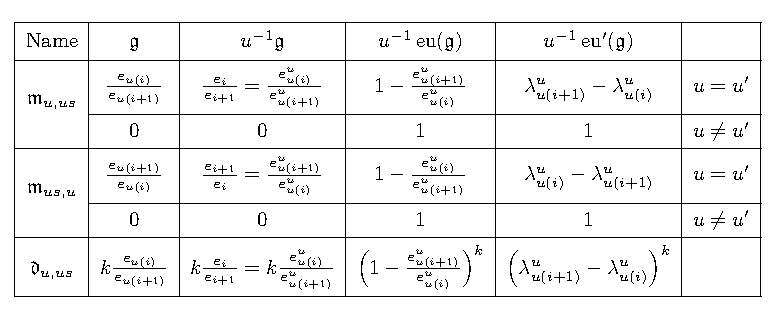
\includegraphics[width=12cm]{figures/table/table_euler_class.pdf}
      \caption{}
      \label{table:euler_class_1}        
\end{table}

Theorem \ref{thm:Demazure_operator_1} is our final destination in this part. We will express its importance in Subsection \ref{subsec:miscellaneous}, see some generalizations in Section \ref{sec:generalization} and compute some examples in Section \ref{sec:diagram}.

\subsection{Miscellaneous}\label{subsec:miscellaneous}
In this subsection, we collect some more results. The arguments in reference work for both $K$-theory and cohomology theory.

\begin{proposition}\label{prop:faithfulness}
The action of $K^{G_{\dimvec{d}}}(\St_{\dimvec{d}})$ on $K^{G_{\dimvec{d}}}(\RRep_{\dimvec{d}}(Q))$ is faithful.
\end{proposition}
\begin{proof}[Sketch of proof]
Reduce the problem to the faithfulness for the action of $\Kcurl^{T_{\dimvec{d}}}(\St_{\dimvec{d}})$ on $\Kcurl^{T_{\dimvec{d}}}(\RRep_{\dimvec{d}}(Q))$. For details, see \cite[Theorem 10.10]{przezdziecki2015geometric}.
\end{proof}

\begin{proposition}\label{prop:generators}
The elements $\{D_{i}^{u,u'}\}_{u,u',i}$ generate $K^{G_{\dimvec{d}}}(\St_{\dimvec{d}})$ as a $K^{G_{\dimvec{d}}}(\RRep_{\dimvec{d}}(Q))$-algebra.
\end{proposition}
\begin{proof}[Sketch of proof]
See \cite[Theorem 11.3]{przezdziecki2015geometric}. The key observation is \cite[Lemma 7.30, 11.4]{przezdziecki2015geometric}.
\end{proof}
Combining these propositions with Theorem \ref{thm:Demazure_operator_1}, we understand the convolution structure of $K^{G_{\dimvec{d}}}(\St_{\dimvec{d}})$ theoretically.